\documentclass{standalone}
\usepackage{PhysicalChemistryNote}
\begin{document}
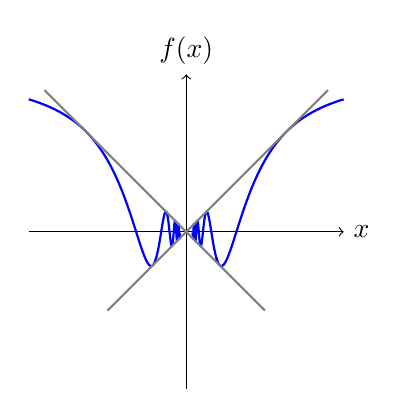
\begin{tikzpicture}[scale=2]
	\draw[->] (-1,0)--(1,0) node[right]{$x$};
	\draw[->] (0,-1)--(0,1) node[above]{$f(x)$};
	\draw[-,blue,thick,domain=-1:-0.19]plot[samples=400](\x,{\x*sin(180/(\x*pi))});
	\draw[-,blue,thick,domain=-0.2:-0.04]plot[samples=1000](\x,{\x*sin(180/(\x*pi))});
	\draw[-,blue,thick,domain=0.19:1]plot[samples=400](\x,{\x*sin(180/(\x*pi))});
	\draw[-,blue,thick,domain=0.04:0.2]plot[samples=1000](\x,{\x*sin(180/(\x*pi))});
	\draw[-,thick,gray,domain=-0.5:0.9] plot[smooth](\x,\x);
	\draw[-,thick,gray,domain=-0.9:0.5] plot[smooth](\x,-\x);
\end{tikzpicture}
\end{document}
\end{document}